\documentclass[twocolumn,twoside,9.5pt]{jarticle}
\usepackage[dvipdfmx]{graphicx}
\usepackage{picins}
\usepackage{fancyhdr}
%\pagestyle{fancy}
\lhead{\parpic{
\includegraphics[height=1zw,keepaspectratio,bb=0 0 251 246]{pic/emblem-bitmap.pdf}}琉球大学主催 工学部工学科知能情報コース 中間発表予稿}
\rhead{}
\cfoot{}

\setlength{\topmargin}{-1in \addtolength{\topmargin}{15mm}}
\setlength{\headheight}{0mm}
\setlength{\headsep}{5mm}
\setlength{\oddsidemargin}{-1in \addtolength{\oddsidemargin}{11mm}}
\setlength{\evensidemargin}{-1in \addtolength{\evensidemargin}{21mm}}
\setlength{\textwidth}{181mm}
\setlength{\textheight}{261mm}
\setlength{\footskip}{0mm}
\pagestyle{empty}

\begin{document}
\title{CNNを用いた楽曲の感情分類\\Emotional classification of songs using CNN}
\author{学籍番号 {175720C} 氏名 {松田理美} 指導教員 : 山田孝治}
\date{}
\maketitle
\thispagestyle{fancy} 

\section{はじめに}
音楽を聴いた時,人は楽しい気分になったり,その曲に荘厳さを感じたりする.これは\cite{ogushi}に述べられているように,音楽と感情が深い関係にあるからである.音楽を聴いて何か特定の感情を得たいという際に,その感情を得ることができる楽曲を選ぶことになるが,その為には既にその楽曲を聴いたことがある前提となる.そのため,新しい楽曲を開拓していくことは難しい.\\
 現在のApple Musicなどにある楽曲検索システムでは,オススメと表示される楽曲は,最近聴いていた楽曲のアーティストの別の楽曲などが表示されるが,同じアーティストでも曲の雰囲気が違うことはあり得るので,求める楽曲が並ばないことがある.オススメされた楽曲をお気に入り楽曲として登録していくことで,自分の求める楽曲を集めていくことはできるが,その楽曲を一度聴いてから判断する必要があるので,時間がかかってしまう.\\
 \cite{gushiken1},\cite{gushiken2}では,楽曲の歌詞に注目して,歌詞情報に基づく楽曲聴取者の気分に応じた楽曲推薦システムの実現を目指していた.歌詞から取得した感情単語を元に,楽曲の感情分類を行なっていたが,評価実験を行うにあたって,楽曲を実際被験者に聴取させ,5種類の感情の中から1つ以上を選択する形を採っていた.しかし,実際に楽曲を聴くことになるので,楽曲の持つメロディで判断している可能性があった.\\
 そこで本研究では,楽曲のメロディのみに注目し,メロディのみでも感情分類が行えるかを調査するために,メロディ情報に基づく楽曲聴取者の気分に応じた楽曲推薦システムの実現を目指す.\\
 先行研究で行われた,音声ファイルの波形から特徴量を抽出し,CNNを利用して分類する研究を元に,楽曲聴取者が感じた感情と比較し,メロディを情報を元にした教師あり学習による楽曲の分類を行う.
\section{先行研究}
\subsection{楽曲の特徴量}
\cite{deep}では,楽曲に使われている楽器を判別する為に,メル周波数スペクトログラムを抽出し,離散コサイン変換(DCT)をかけて,各楽器のメル周波数ケプストラム係数(MFCC)を抽出し,CNNを利用して分類を行なっていた.しかし,DCTを行うと,特定の周波数帯の特徴量のみを残し,他の周波数帯の特徴量を消すため,楽曲内に使われている特定の楽器を判別することなどは可能だが,楽曲の特徴の大部分が削除されてしまうため,楽曲全体を利用した学習が不可能になってしまう.\\
 下の図\ref{f1},図\ref{f2}は,Runner Runnerの楽曲,「So Obvious」という楽曲の冒頭から1分間を,メル周波数スペクトログラムの抽出までを行なった画像と,MFCCの抽出までを行なった画像である.\\
 横軸は時間,縦軸は周波数,色の濃さはその時間のその周波数帯での音圧を表しており,色が薄いほど音圧が高いことを表している.\\\
\begin{figure}[htbp]
	\includegraphics[width=100mm]{pic/melsample.pdf}
	\caption{メル周波数スペクトログラム}
	\label{f1}
\end{figure}
\begin{figure}[htbp]
	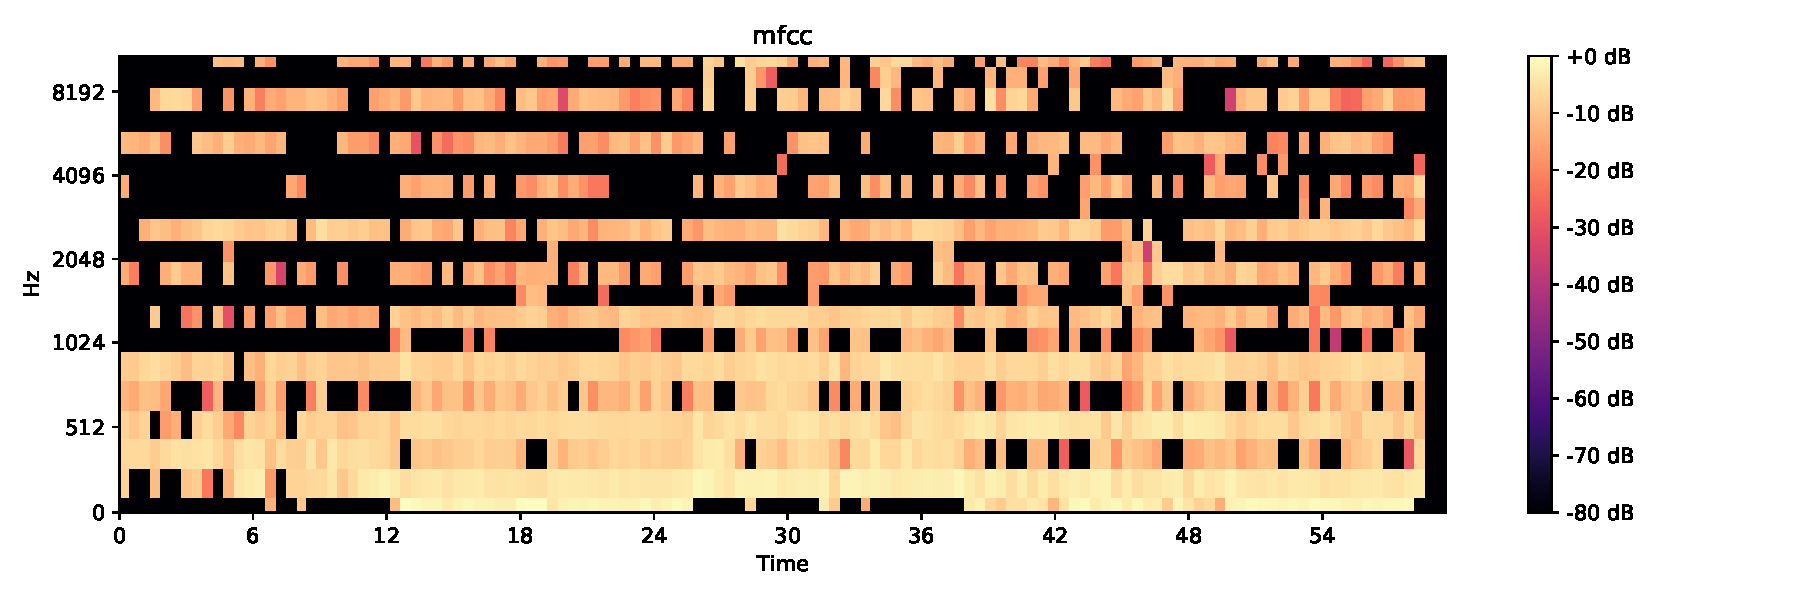
\includegraphics[width=100mm]{pic/mfccsample.pdf}
	\caption{図\ref{f1}にDCTを行なって抽出したMFCC}
	\label{f2}
\end{figure}
\\
 この楽曲は,最初の約12秒間は落ち着いたメロディーだが,そこから約12秒間少し激しい曲調へと変わり,また落ち着いたメロディーへと戻っていく.\\
 図\ref{f1}では,最初の約12秒間は全体的に低い音圧から始まり,そこからまた約12秒間高い音圧になっていることを表しており,その後また低い音圧へと戻っている.\\
 対して,図\ref{f2}では,ほぼ常に高い音圧が出続けているような状態を表しており,主に高い周波数帯で音圧がほぼ0に近い状態になっている.\\
 本研究では,メル周波数スペクトログラムにDCTを行う手順を省き,メル周波数スペクトログラムをそのままCNNに利用する.
\subsection{感情カテゴリー}
\cite{gushiken1},\cite{gushiken2}での実験での感情分類の結果と比較を行う為に,同じ5つの感情カテゴリーに分ける.感情カテゴリーは,喜び,安らぎ,悲しみ,昂り,好意の5つである.
\section{提案手法}
\cite{deep}での特徴量の抽出の手法と,\cite{gushiken1},\cite{gushiken2}での感情分類に利用された感情カテゴリーを利用し,以下の手順で波形分類を行う.

\subsection{アンケート}
被験者が普段聴取している楽曲からランダムに50曲を選択.それらの楽曲のメロディーのみを実際に聴いてもらい,その楽曲の印象を感情カテゴリーの5つの中から選択してもらう.選択された感情を,正解ラベルとする.\\

\subsection{特徴量の抽出}
データ量を増やす為に,1曲を1分ごとに分割し,楽曲のメル周波数スペクトログラムを抽出する.\\

\subsection{モデルの作成}
アンケートによって集計したデータセットのうち,40曲分の画像データを訓練データとして学習し,10曲分の画像をテストデータとして使用する.\\


\section{今後の課題}
本研究を行う為に,被験者へのアンケート調査による楽曲の収集及び正解ラベルの作成,学習を行う為のCNNの実装などを早急に行う必要がある.\\


\begin{thebibliography}{9}

\bibitem{ogushi} 音楽と感情, 大串健吾, 2006
\bibitem{gushiken1} 歌詞情報を用いた楽曲の推薦システム, 具志堅大輝, 山田孝治, 2019
\bibitem{gushiken2} 歌詞情報を用いた歌詞の楽曲分類手法, 具志堅大輝, 山田孝治, 2020
\bibitem{deep} DEEP CONVOLUTIONAL NETWORKS ON THE PITCH SPIRAL FOR MUSICAL INSTRUMENT RECONGNITION, Vincent Lostanlen and Carmine-Emanuele Cella,\'{E}cole normale sup\'{e}rieure, PSL Research University, CNRS, Paris, France, 2017
\bibitem{proc} Deep Learning for Audio Signal Processing, Hendrik Purwins, Bo Li, Tuomas Virtanen, Jan Schl\H{u}ter, Shuo-yiin Chang, Tara Sainath, 2019
\bibitem{kate} Experimental Studies of the Elements of Expression in Music, Kate Hevner, 2020
\bibitem{huruya1} 古屋瑞生・黄宏軒・川越恭二(2014)「歌詞情報に基づく 聴取目的に応じた楽曲推薦システムの提案」, 情報処理 学会第 76 回全国大会
\bibitem{huruya2} 聴取目的に応じた音楽推薦のための歌詞からの音楽印象 分類方法, 古屋瑞生・黄宏軒・川越恭二, 2015


\end{thebibliography}
\end{document}
